\section{Transient subtraction method}
\label{sec:transient}
%
We propose in this section a method called \emph{transient subtraction technique}, which employs a subtraction technique similar to the one suggested in \cite{ciccotti1975} to the transient dynamics method discussed in Section \ref{subsec:transient} as a means for variance reduction. We first outline in Section \ref{subsec:constructing_method} the construction of the method, then present the numerical analysis of its associated estimators in Section \ref{subsec:num_anal_ts}.

\subsection{Constructing the method}
\label{subsec:constructing_method}
%
In the transient dynamics setting of Section~\ref{subsec:transient}, one can consider the use of couplings as a control variate approach to construct an estimator with lower variance than~\eqref{eq:T_estimator}. To this end, we consider the coupling $(X_t^\eta,Y_t^0)$, where the processes $X_t^\eta$ and $Y_t^0$ are evolved according to the same underlying reference dynamics and have different initial conditions:
%
\begin{equation}
\begin{cases}
\begin{aligned}
	dY_t^0 &= b(Y_t^0) \, dt + \sigma \, dW_t, \qquad Y_0^0 \sim \mu, \\
	dX_t^\eta &= b(X_t^\eta) \, dt + \sigma \, d\widetilde{W}_t, \qquad X_0^\eta \sim \psip,
\end{aligned}
\end{cases}
\label{eq:coupled_dynamics}
\end{equation}
%
where $W_t$ and $\widetilde{W}_t$ are standard $m$-dimensional Brownian motions. The transport coefficient $\rho$ can then be computed as
%
\begin{equation}
%	\rho = \lim_{\eta\to 0} \frac{1}{\eta}\int_0^{+\infty} \E\left(R(X_t^\eta) - R(Y_t^0)\right) dt,
	\rho = \lim_{\eta\to 0} \frac{1}{\eta}\int_0^{+\infty} \E\paren*{R(X_t^\eta) - R(Y_t^0)}\,  dt.
	\label{eq:tc_subtraction}
\end{equation}
%
Note that $\int_0^{+\infty} R(Y_t^0) \, dt$ acts as a control variate since $\E(R(Y_t^0))=0$ for all $t\geq 0$. The expression~\eqref{eq:tc_subtraction} admits the following natural estimator, carried out with independent initial conditions for the couple $(X_t^{\eta,k},Y_t^{0,k})_{t\geq 0}$ for $1\leq k\leq K$ and independent realizations of the dynamics~\eqref{eq:coupled_dynamics}:
%
\begin{equation}
    \TSest = \frac{1}{\eta K} \sum_{k=1}^K \int_0^T \bkt*{R(X_t^{\eta,k}) - R(Y_t^{0,k})} \, dt.
    \label{eq:ts_estimator}
\end{equation}
%
A sufficient condition for \eqref{eq:ts_estimator} to have smaller variance than the standard estimator \eqref{eq:T_estimator} is for the trajectories to start $\eta$ close, and to stay close for times of order $1/\lambda$, where $\lambda$ is the relaxation rate of the system to the stationary state (see \cref{as:decay_semigroup}). More precisely,
%
%To ensure that \eqref{eq:ts_estimator} has smaller variance than the standard estimator \eqref{eq:T_estimator}, two conditions must be fulfilled: %we need the difference~$|X_t^\eta - Y_t^0|$ to start and remain $\bigO(\eta)$. This suggests that the coupling is comprised of two parts: 

\begin{enumerate}[label={(\Alph*)}]
	\item \label{enum:init_dist} The initial distance $|X_0^\eta - Y_0^0|$ must be of order $\eta$;
	\item \label{enum:stay_close} The dynamics must remain $\eta$ close for finite times as the copies of the system evolve, i.e.\ $|X_t^\eta - Y_t^0|$ must be of order $\eta$ for $t\leq T$.
\end{enumerate}
%
Condition \ref{enum:init_dist} amounts to finding a coupling measure which is concentrated along the diagonal in the~$(x,y)$ space, so that initial conditions are $\eta$ close. We emphasize that, although $\psip$ is by construction a $\bigO(\eta)$ perturbation of~$\mu$, this is not enough to guarantee that the trajectories start $\eta$ close when the initial conditions are independent, thus we require a coupling on the initial conditions.

 We discuss in Section \ref{subsubsec:synchronous_coup} a natural way of coupling the dynamics \eqref{eq:coupled_dynamics}, and outline sufficient conditions for condition \ref{enum:stay_close} to hold. Then, we formally construct the coupling measure on the initial conditions and discuss its properties in Section \ref{subsubsec:properties_init_cond}.
 
\begin{remark}[{\bf Tangent dynamics}]
%
The expression \eqref{eq:tc_subtraction} of the transport coefficient can be formulated in terms of tangent dynamics \cite{assaraf2017}. Denote by $\mathcal{T}_t\in\R^d$ the tangent vector, where
%
\begin{equation}
	\mathcal{T}_t 
%	= \partial_\eta^0 X_t^\eta 
	= \lim_{\eta\to 0} \frac{X_t^\eta - X_t^0}{\eta}.
\end{equation} 
%
This vector evolves according to a random ordinary differential equation, obtained by linearizing \eqref{eq:general_SDE}. Moreover,
%Then, since $\partial_\eta^0 R(X_t^\eta) = \mathcal{T}_t\cdot \nabla R(X_t^0)$, 
\eqref{eq:tc_subtraction} can be written as
%
\begin{equation}
	\rho = \lim_{\eta\to 0} \frac{1}{\eta}\int_0^{+\infty} \E\paren*{R(X_t^\eta) - R(Y_t^0)} \, dt = \int_0^{+\infty} \E\paren*{\mathcal{T}_t\cdot \nabla R(X_t^0)} \, dt.
\end{equation}
%
\end{remark}

\subsubsection{Synchronous coupling}
\label{subsubsec:synchronous_coup}
%
A natural way to ensure that the dynamics remain close is via synchronous coupling, which amounts to using the same Brownian motion for both processes, i.e.\ setting $\widetilde{W} = W$. It is known that synchronous coupling performs well in the presence of global dissipativity. Without it, however, trajectories decouple and we cannot control the coupling distance for long times. For the transient subtraction method, we do not require long-time results, as the relaxation time of the estimator~\eqref{eq:ts_estimator} is typically of order $\bigO(1/\lambda)$, with $\lambda$ the exponential convergence rate from \cref{as:decay_semigroup}. Thus, this suggests that synchronous coupling is an admissible control variate as long as the relaxation time is smaller than the decoupling time.

In order to more precisely state some results on the coupling distance, we give a sufficient condition for trajectories to decouple at most exponentially in time in \cref{as:contractivity}. % We assume the drift $b$ to be such that the following assumption holds.
 
\begin{assumption}
\label{as:contractivity}
	There exists $B\in\R$ such that the drift $b\colon \mathcal{X} \to \R^d$ satisfies
	%
	\begin{equation}
		\forall (x,y) \in \mathcal{X}^2, \qquad \langle x-y, b(x)-b(y)\rangle \leq B|x-y|^2.
		\label{eq:no_dissip}
	\end{equation}
	%
	
\end{assumption}

A sufficient condition for \eqref{eq:no_dissip} to be satisfied is when the drift $b$ is globally Lipschitz with constant~$\bLip$, in which case $B = \bLip$. In some fortunate cases where $B<0$, the drift is globally dissipative. In particular, global dissipativity ensures uniform exponential decay of the coupling distance $|X_t^\eta - Y_t^0|$.  % In other words, the drift constraints the trajectories to some compact region around the origin
%
We next state a standard result providing an upper bound for how fast trajectories decouple based on the estimate considered in \Cref{as:contractivity}.

\begin{lemma}
	\label{lemma:decoupling_times}
	Suppose that \Cref{as:contractivity} holds. Then, almost surely,
	%
	\begin{equation}
%	|X_t^\eta - Y_t^0|^2 \leq \e^{2tB}|X_0^\eta - Y_0^0|^2.
		\forall t\geq 0, \qquad |X_t^\eta - Y_t^0| \leq \e^{tB}|X_0^\eta - Y_0^0|.
	\label{eq:gronwall_decouple}
	\end{equation}
	%
\end{lemma}

\begin{proof}%[Proof of Lemma \ref{lemma:decoupling_times}]
	In order to bound the distance between the trajectories at time $t$ in terms of the initial distance, we first write, by It\^o's formula
	%
	\begin{align}
		d\bigl(|X_t^\eta - Y_t^0|^2\bigr) &= 2\ip{X_t^\eta - Y_t^0, dX_t^\eta - dY^0_t} \\
		&= 2\langle X_t^\eta - Y_t^0, b(X_t^\eta) - b(Y_t^0)\rangle \, dt \\
		&\leq 2B|X_0^\eta - Y_0^0|^2 \, dt.
		\label{eq:ito_dissip}
	\end{align}
	%
	Gr\"onwall's lemma then gives the claimed bound. %\red{maybe add some formal details on gronwall?}
	%
\end{proof}

%\begin{proof}[(Gr\"onwall) Proof of Lemma \ref{lemma:decoupling_times}]
%	In order to bound the distance between the trajectories at time $t$ in terms of the initial distance, we first write, by It\^o's formula
%	%
%	\begin{align}
%		d\bigl(|X_t^\eta - Y_t^0|^2\bigr) &= 2\langle X_t^\eta - Y_t^0, b(X_t^\eta) - b(Y_t^0)\rangle.
%	\end{align}
%	%
%	We can now apply Gr\"onwall's inequality to \eqref{eq:ito_dissip} for each case in \Cref{as:contractivity}, which leads to
%%	
%	\begin{itemize}
%		\item No dissipativity \ref{cond:no_dissip}: $d\bigl(|X_t^\eta - Y_t^0|^2\bigr) \leq 2B|X_t^\eta - Y_t^0|^2.$
%%		%
%%		\begin{equation}
%%			d\bigl(|X_t^\eta - Y_t^0|^2\bigr) \leq 2B|X_t^\eta - Y_t^0|^2.
%%			\label{eq:ineq_no_dissip}
%%		\end{equation}
%		%
%		\begin{align}
%			|X_t^\eta - Y_t^0|^2 &\leq \e^{2tB}|X_0^\eta - Y_0^0|^2.
%%			\label{eq:gronwall_no_dissip}
%		\end{align}
%		
%		\item Dissipativity at infinity \ref{cond:dissip_at_infty}: $d\bigl(|X_t^\eta - Y_t^0|^2\bigr) \leq -2B|X_t^\eta - Y_t^0|^2 + 2A.$
%		%
%%		\begin{equation}
%%			d\bigl(|X_t^\eta - Y_t^0|^2\bigr) \leq -2B|X_t^\eta - Y_t^0|^2 + 2A.
%%			\label{eq:ineq_dissip_at_infty}
%%		\end{equation}
%%		%
%		\begin{align}
%			|X_t^\eta - Y_t^0|^2 &\leq \e^{-2tB}|X_0^\eta - Y_0^0|^2 + \frac{A}{B}(1 - \e^{-2Bt}).
%%			\label{eq:gronwall_dissip_at_infty}
%		\end{align}
%		
%		\item Dissipativity \ref{cond:dissip}: $d\bigl(|X_t^\eta - Y_t^0|^2\bigr) \leq -2B|X_t^\eta - Y_t^0|^2.$
%		%
%%		\begin{equation}
%%			d\bigl(|X_t^\eta - Y_t^0|^2\bigr) \leq -2B|X_t^\eta - Y_t^0|^2.
%%			\label{eq:ineq_dissip}
%%		\end{equation}
%		%
%		\begin{align}
%			|X_t^\eta - Y_t^0|^2 &\leq \e^{-2tB}|X_0^\eta - Y_0^0|^2.
%%			\label{eq:gronwall_dissip}
%		\end{align}
%	\end{itemize}
%	%
%	which concludes the proof.
%\end{proof}
%
%Although the dynamics eventually decouple, there are conditions under which the control variate is still effective in reducing the variance of \eqref{eq:ts_estimator}. This is the case for instance when $B>0$ is small enough compared to the convergence of $\e^{t\L}R$ to 0, so that relaxation occurs faster than decoupling.

\subsubsection{Properties of initial conditions}
\label{subsubsec:properties_init_cond}
%
We consider a coupling measure $\mucoup(dx \, dy)$ with marginals $\psip(dx)$ and $\mu(dy)$. In order to ensure that the initial conditions are $\eta$ close, the coupling measure must be concentrated along the diagonal (more precisely, within $\eta$ distance from the diagonal), as illustrated in \cref{fig:coup_meas_mock}. A natural way of achieving this is to formulate~$X_0^\eta$ as a deterministic map of $Y_0^0$, i.e.\ to look for $\Phi_\eta \colon \mathcal{X} \to \mathcal{X}$ such that~$X_0^\eta = \Phi_\eta(Y_0^0)$, with~$\Phi_\eta$ close to the identity function. The function~$\Phi_\eta$ should be chosen such that
%
\begin{equation}
	\psip = \Phi_\eta \# \mu = (1+\eta S)\mu + \bigO(\eta^2),
	\label{eq:deterministic_map}
\end{equation}
%
where $\#$ denotes the image measure of $\mu$ by $\Phi_\eta$: For any bounded measurable test function~$\varphi\colon \X \to \R$,
%
\begin{equation}
	\int_\mathcal{X} \varphi \, d\psip = \int_\mathcal{X} \varphi \circ \Phi_\eta \, d\mu.
\end{equation}
%
We look for a map $\Phi_\eta$ of the form
%
\begin{equation}
	\Phi_\eta(x) = x + \eta\varphi_1(x),
	\label{eq:Phi_map}
\end{equation}
%
%where $\varphi_1$ has to be chosen so that it coincides with $\psip$ up to order $\eta$, 
where $\varphi_1$ is determined by \eqref{eq:deterministic_map}. It is in fact given by a solution to the partial differential equation (PDE) \eqref{eq:varphi1_PDE} below, as made precise in \cref{prop:gen_subtraction}.
%
Note that \eqref{eq:Phi_map} can be formulated as a map higher than first-order in $\eta$; see \cref{subsubsec:bias_analysis} for a discussion of this point.

The transient subtraction technique then amounts to evolving synchronously coupled equilibrium dynamics starting from initial conditions which are deterministically related:
%
\begin{equation}
\begin{cases}
\begin{aligned}
	dY_t^0 &= b(Y_t^0) \, dt + \sigma \, dW_t, \qquad Y_0^0 \sim \mu, \\
	dX_t^\eta &= b(X_t^\eta) \, dt + \sigma \, dW_t, \qquad X_0^\eta = \Phi_\eta(Y_0^0).
\end{aligned}
\end{cases}
\label{eq:sub_dyn}
\end{equation}
%
We next perform error analysis on the transient subtraction technique estimator \eqref{eq:ts_estimator} for~$(X_t^\eta)_{t\geq 0}$ and~$(Y_t^0)_{t\geq 0}$ given by~\eqref{eq:sub_dyn}.
 
\begin{figure}%[H]
	\centering
	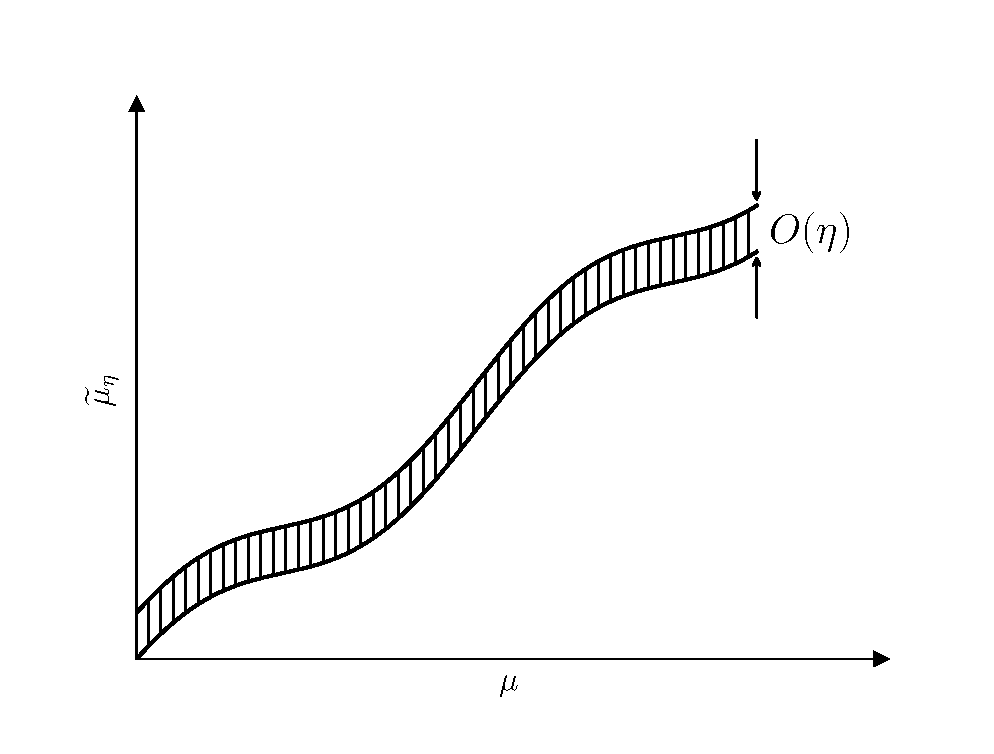
\includegraphics[width=0.75\textwidth]{coup_meas_plot.eps}
	\caption{Illustration of coupling measure on initial conditions.}
	\label{fig:coup_meas_mock}
\end{figure}

\subsection{Numerical analysis of the transient subtraction method}
\label{subsec:num_anal_ts}
%
In this section, we perform error analysis on the transient subtraction estimator \eqref{eq:ts_estimator} realized with the dynamics~\eqref{eq:sub_dyn}. We start by making precise the functional setting and stating some estimates in \cref{subsubsec:lyapunov_setting}. We then make precise in Section \ref{subsubsec:bias_analysis} the bounds on the bias, and finally discuss its variance in Section \ref{subsubsec:variance_analysis}.
%Before stating the technical results, we must first define some necessary \red{functional setting}, required to make precise the analysis done in this section.

\subsubsection{Functional estimates}
\label{subsubsec:lyapunov_setting}
%
Consider a family of Lyapunov functions $(\mathcal{K}_n)_{n\in\N}$ with $\mathcal{K}_n \colon \mathcal{X} \to [1,+\infty)$ such that
%
\begin{equation}
	\forall n\in\N, \qquad \mathcal{K}_n \leq \mathcal{K}_{n+1}.
\end{equation}
%
The associated weighted $B^\infty$ spaces are
%
\begin{equation}
    B_n^\infty = \left\{\varphi \, \rm{measurable} \; \middle| \; \|\varphi\|_{B_n^\infty} := \sup _{x \in \mathcal{X}}\left| \frac{\varphi(x)}{\mathcal{K}_n(x)} \right| < +\infty\right\}.
\end{equation}
%
We next introduce the space $\S$ of smooth functions $\varphi$ belonging to the space $B^\infty_n$ for some $n$, and whose derivatives also belong to $B^\infty_m$ for some $m$:
%
\begin{equation}
    \S = \left\{\varphi \in C^\infty(\mathcal{X}) \; \middle| \; \forall k \in \mathbb{N}^d, \; \exists n \in \mathbb{N}, \; \partial^k \varphi \in B_n^\infty\right\}.
\end{equation}
%
We finally define the subspace $\S_0$ of functions in $\S$ with average 0 with respect to $\mu$.

We make the following assumptions on the Lyapunov functions.

\begin{assumption}[{\bf Lyapunov estimates}]
\label{as:lyapunov}
%
%The identity belongs to $B^\infty_n$: t
There exist $n\in\N$ and~$C_n\in\R^+$ such that
%
\begin{equation}
	|x| \leq C_n\mathcal{K}_n(x).
	\label{eq:lyap_identity}
\end{equation}
%
%Furthermore, the space $\S$ is dense in $L^2(\mu)$. In particular, for any $n\in\N$, there exists $M_n$ such that
Furthermore, for any~$n\in\N$,
%
\begin{equation}
	\norm{\mathcal{K}_n}_{L^1(\mu)} < +\infty.
	\label{eq:lyap_L1}
\end{equation}
%
Moreover, we assume that the Lyapunov functions are stable by products: for any~$n,n'\in\N$, there exist~$m\in\N$ and $C_{n,n'}\in\R^+$ such that
%
\begin{equation}
	\paren*{\mathcal{K}_n\mathcal{K}_{n'}}(x) \leq C'_{n,n'}\mathcal{K}_m(x).
	\label{eq:lyap_prod}
\end{equation}
%
We also assume stability by compositions: for any~$n,n'\in\N$ and~$\alpha^*\in\R^+$, there exist~$m\in\N$ and~$C_{n,n',\alpha^*}\in\R^+$ such that
%
\begin{equation}
	\forall\alpha \in [0,\alpha^*], \qquad \mathcal{K}_n(\alpha\mathcal{K}_{n'}(x)) \leq C_{n,n',\alpha^*}\mathcal{K}_m(x).
	\label{eq:lyap_comp}
\end{equation}
%
Lastly, we assume that $\mathcal{K}_n$ is nondecreasing:
%
\begin{equation}
	\paren*{\forall i = 1,\dotsc,d, \quad |y_i| \leq |z_i|} \implies \mathcal{K}_n(y) \leq \mathcal{K}_n(z).
\end{equation}
%
\end{assumption}

%\begin{remark}
%\label{rem:composition_computation}
%
A useful corollary of \cref{as:lyapunov}, which we will use in our estimates, is the following: for any~$f\in B^\infty_{n}$ and~$g = (g_1,\dotsc,g_d)$ with $g_i \in B^\infty_{n'}$, %there exists $K_{n,n'}\in\R^+$ such that $f\circ g \leq K_{n,n'}\mathcal{K}_m$ since, for nondecreasing~$\mathcal{K}_n$,
%
\begin{align}
	|f\circ g|(x) \leq \|f\|_{B_{n}^\infty}\mathcal{K}_{n} \circ g(x) %\\
	\leq \|f\|_{B_{n}^\infty}\mathcal{K}_{n}\paren*{\|g\|_{B^\infty_{n'}} \mathcal{K}_{n'}(x)} %\\
	\leq \norm{f}_{B^\infty_n}K_{n,n',\|g\|_{B^\infty_{n'}}}\mathcal{K}_{m}(x),
	\label{eq:lyap_composition_cor}
\end{align}
%
with $m$ depending on $n$ and $n'$.
%
%\end{remark}

%For compact spaces $\mathcal{X}$, it suffices to choose $\mathcal{K}_n = 1$ for all $n\in\N$. When $\mathcal{X}$ is unbounded, 
A typical choice for $\mathcal{K}_n$ are polynomial Lyapunov functions of the form $\mathcal{K}_n(x) = 1+|x|^n$. This is a standard choice for Langevin dynamics; see \cite{mattingly2002,talay2002}. This choice satisfies \cref{as:lyapunov} when $\mu$ has moments of all orders, which is a mild requirement.

We also make an assumption on the convergence of the semigroup $\e^{t\L}$ in weighted $B^\infty$ spaces. To this end, we introduce the space $B^\infty_n$ of functions with average 0 with respect to $\mu$:
%
\begin{equation}
    \Binfz = \left\{\varphi \in B^\infty_n \; \middle| \; \int_\mathcal{X} \varphi \, d\mu = 0\right\}.
\end{equation}
%

\begin{assumption}[{\bf Decay estimates on semigroup operator}]
	\label{as:decay_semigroup}
	%
	For any $n\in\N$, there exist~$L_n \in \R^+$ and $\lambda_n>0$ such that
	%
	\begin{equation}
		\forall \varphi\in \Binfz, \qquad \|\e^{t\L}\varphi\|_{B^\infty_n} \leq L_n\e^{-\lambda_n t}\norm{\varphi}_{B^\infty_n}.
%		\|\e^{t\L}\|_{\mathcal{B}(\Binfz)} \leq L_n\e^{-\lambda_n t},
	\label{eq:decay}
	\end{equation}
	%
\end{assumption}
%

%See \cite[Section 2]{lelievre2016} for a discussion on sufficient conditions for the above to hold. 
As a direct corollary of \cref{as:decay_semigroup}, the operator $\L$ is invertible on $\Binfz$, with
%
\begin{equation}
	\L^{-1} = -\int_0^{+\infty} \e^{t\L} \, dt.
	\label{eq:op_identity}
\end{equation}
%
Moreover, the following bound holds
%
\begin{equation}
	\norm{\L^{-1}}_{B^\infty_n} \leq \frac{L_n}{\lambda_n}.
	\label{eq:Linv_bound}
\end{equation}
%
We refer for instance to \cite[Section 2]{lelievre2016} for a discussion on sufficient conditions for \cref{as:decay_semigroup} to hold (based on \cite{reybellet2006,hairer2011}), and for the proof of \eqref{eq:op_identity}. 

\subsubsection{Analysis of the bias}
\label{subsubsec:bias_analysis}
%
There are several sources of bias arising from the estimator~\eqref{eq:ts_estimator}, such as the time truncation and time discretization bias when considering numerical schemes to integrate the dynamics. Quantifying such biases is standard practice for estimators of this form. Additionally, there is a bias arising from the finiteness of $\eta$, which is the main result of this section. This is made precise in \cref{cor:gk_equiv}, which builds upon the estimates on the coupling measures provided by~\cref{prop:gen_subtraction} below. 

To state the result, we denote by $\mathcal{A}^*$ the adjoint of a closed operator $\mathcal{A}$ on $L^2(\mu)$: for any test functions~$\varphi, \phi \in C^\infty$ with compact support,
%
\begin{equation}
    \int_\mathcal{X} (\mathcal{A}\varphi)\phi \, d\mu = \int_\mathcal{X} \varphi(\mathcal{A}^*\phi) \, d\mu.
    \label{eq:Astar_adjoint}
\end{equation}
%
%
%We first state a formal result which makes precise the bias associated with the deterministic map \eqref{eq:Phi_map}, and the derivation of some relevant PDEs.

%\tmpbox{
%\begin{remark}[\red{TEMP: Taylor Lagrange remainder}]
%	Let $\Phi_\eta(x) = x+\eta\varphi_1(x)+\eta^2\varphi_2(x)$,
%	%
%	\begin{align}
%		f(\Phi_\eta(x)) = f(x) + \Phi_\eta(x)^T \nabla f + \frac{1}{2}\Phi_\eta(x)^T\nabla^2f\Phi_\eta(x) + R_3
%	\end{align}
%	%
%	with
%	%
%	\begin{equation}
%		R_3 = \frac{1}{6}D^3f\left((1-\theta)x + \theta\Phi_\eta\right)\cdot \Phi_\eta(x)^{\otimes 3}
%		\label{eq:remainder_og_form}
%	\end{equation}
%	%
%	In integral form, \red{to be double checked}
%	%
%	\begin{equation}
%		R_3 = \frac{(\Phi_\eta - x)^3}{2}\int_0^1 (1-t)^2 D^3f((1-t)x + t\Phi_\eta) \, dt
%		\label{eq:remainder_int_form}
%	\end{equation}
%	%
%	\red{don't think we need \eqref{eq:remainder_int_form}. I think \eqref{eq:remainder_og_form} is enough for the proofs since it's already inside integral, so we can use lyapunov estimates to bound everything}
%\end{remark}}

\begin{proposition}[{\bf Finite $\eta$ bias}]
\label{prop:gen_subtraction}
%
Suppose that \cref{as:lyapunov} holds true and that, for $S\in\S_0$, there exist solutions $\varphi_1 = (\varphi_{1,x_1},\dotsc,\varphi_{1,x_d}) \in (B^\infty_n)^d$ and $\varphi_2=(\varphi_{2,x_1},\dotsc,\varphi_{2,x_d}) \in (B^\infty_n)^d$ for some $n\in\N$ to the equations
%
\begin{equation}
	\nabla^*\varphi_1 = \sum_{i=1}^d \partial_{x_i}^* \varphi_{1,x_i} = S, %-\div(\varphi_1) + \beta\nabla U\varphi_1 = S
	\label{eq:varphi1_PDE}
\end{equation}
%
and
%
\begin{equation}
	\nabla^*\varphi_2 = -\frac{1}{2}\sum_{i,j=1}^d \partial_{x_i}^*\partial_{x_j}^* (\varphi_{1,x_i}\varphi_{1,x_j}) = -\frac{1}{2}(\nabla^*)^2 \colon \varphi_1\otimes \varphi_1.
	\label{eq:varphi2_PDE}
\end{equation}
%
Fix $\eta_*>0$, and $f\in \S$. Then, there exists $K_{f,\eta_*} \in\R_+$ (which depends on~$f$ and~$\eta_*$) such that, for any~$|\eta| \leq \eta_*$,
%
\begin{equation}
	\qquad \left|\int_\mathcal{X} f\circ\Phi^\alpha_\eta \, d\mu - \int_\mathcal{X} f \, d\mu - \eta\int_\mathcal{X} f S \, d\mu\right| \leq \eta^{\alpha+1} \mathcal{C}_{f,\eta_*},
	\label{eq:prop_eta_bias_bound}
\end{equation}
%
with $\alpha=1$ or $\alpha=2$, and
%
\begin{equation}
\begin{cases}
\begin{aligned}
	&\Phi_\eta^1(x) = x + \eta\varphi_1(x), \\
	&\Phi_\eta^2(x) = x + \eta\varphi_1(x) + \eta^2\varphi_2(x).
\end{aligned}
\end{cases}
\label{eq:Phi_alpha}
\end{equation}
%
\end{proposition}

\begin{remark}
The smoothness condition on $f$ can be weakened, as it would be enough to have derivatives of $f$ up to order 3 in $B^\infty_m$. In order to simplify the presentation of the result, however, we suppose~$f\in \S$ here.
\end{remark}

This result states that the finite $\eta$ bias in the linear response is of order~$\bigO(\eta^{\alpha})$ for a map $\Phi_\eta$ which includes well-chosen terms up to order $\bigO(\eta^\alpha)$. It is of course possible to construct higher-order corrections in order to further decrease the bias. The associated PDEs for the corresponding $\varphi_i$ terms, however, become increasingly cumbersome to solve, rendering it an impractical approach. In any case, a second-order map leads to an estimator with $\bigO(\eta^2)$ bias, which is sufficiently small in general.

\begin{remark}[{\bf Well-posedness of PDEs}]
Although \eqref{eq:varphi1_PDE} might look difficult to solve, one can show that it admits gradient solutions of the form $\varphi_1 = \nabla\psi$ under some conditions on $\mu$. Indeed, \eqref{eq:varphi1_PDE} can then be written as
%
\begin{equation}
	\nabla^*\nabla \psi = S, %\quad (= \Delta \psi + \beta \nabla U^\t \nabla\psi),
\end{equation}
%
which has a unique solution when $\nabla^*\nabla$ has a spectral gap when considered as an operator on~$L^2(\mu)$ (implied by $\mu$ satisfying a Poincar\'e inequality).%, so that $(\nabla^*\nabla)^{-1}$ is well-defined on the space~$L^2_0(\mu)$).
Note that the solutions $\varphi_1$ and $\varphi_2$ are defined up to an element of the kernel of $\nabla^*$, i.e.\ if $\nabla\psi$ is a solution to~\eqref{eq:varphi1_PDE}, then~$\varphi_1 = \nabla\psi + g$ with $\nabla^*g = 0$ also an admissible solution. %Ideally, one would take take the minimum norm solution, or take a specific solution of gradient form.
\end{remark}

\begin{proof}[Proof of Proposition \ref{prop:gen_subtraction}]
It suffices to prove the result for $\alpha=2$, from which the result for $\alpha=1$ can be trivially deduced. By a Taylor expansion of $f(\Phi_\eta(x))$,
%
\begin{align}
		f(\Phi_\eta(x)) = f(x) &+ \eta \nabla f(x)^\t(\varphi_1(x) + \eta\varphi_2(x)) \\
		&+ \frac{\eta^2}{2}(\varphi_1(x) + \eta\varphi_2(x))^\t \nabla^2 f(x)(\varphi_1(x) + \eta\varphi_2(x)) \\
		&+ \frac{\eta^3}{6} \nabla^3f\left(\Theta_\eta(x)\right)\cdot (\varphi_1(x) + \eta\varphi_2(x))^{\otimes 3},
\end{align}
%
where $\nabla^3 f$ % = \nabla \otimes (\nabla^{2} f)$
denotes the third-order derivative tensor (and $\nabla^2 f$ denotes the Hessian), and~$\Theta_\eta(x)$ interpolates between~$x$ and~$\Phi_\eta(x)$:
%
\begin{equation}
	\Theta_\eta(x) = (1-\theta_\eta(x))x + \theta_\eta(x)\Phi_\eta(x), \qquad \theta_\eta(x) \in [0,1].
\end{equation}
%
Integrating the Taylor expansion above yields
%
\begin{align}
	\int_\mathcal{X} f\circ\Phi_\eta \, d\mu &= \int_\mathcal{X} f \, d\mu + \eta \int_\mathcal{X}\nabla f^\t \varphi_1 \, d\mu + \eta^2\int_\mathcal{X} \paren*{\varphi_2^\t \nabla f+\frac{1}{2}\varphi_1^\t(\nabla^2 f)\varphi_1} \, d\mu + \eta^3\mathcal{R}_{3,\eta},
	\label{eq:prop_rhs_terms}
\end{align}
%\begin{align}
%	\begin{split}
%	\int_\mathcal{X} f\circ\Phi_\eta \, d\mu &= \int_\mathcal{X} f \, d\mu + \int_\mathcal{X} \nabla f^\t(\Phi_\eta(x) - x) \, d\mu \\ &\qquad + \frac{1}{2}\int_\mathcal{X} (\Phi_\eta(x) - x)^\t \nabla^2f (\Phi_\eta(x) - x) \, d\mu + \eta^3\mathcal{R}_{3,\theta}
%	\end{split} \\
%	&= \int_\mathcal{X} f \, d\mu + \eta \int_\mathcal{X}\nabla f^\t \varphi_1 \, d\mu + \eta^2\int_\mathcal{X} \left(\varphi_2^\t \nabla f+\frac{1}{2}\varphi_1^\t\nabla^2 f\varphi_1\right) d\mu + \eta^3\mathcal{R}_{3,\theta},
%	\label{eq:prop_rhs_terms}
%\end{align}
%
with $\mathcal{R}_{3,\eta}$ given by %\red{(writing $\Phi_\eta - x$ instead of $\eta\varphi_1+\eta^2\varphi_2$)}
%
\begin{equation}
%	\mathcal{R}_{3,\theta} = \frac{1}{6\eta^3}\int D^3f\left(\Theta_\eta(x)\right)\cdot (\Phi_\eta(x) - x)^{\otimes 3} \, d\mu,
	\mathcal{R}_{3,\eta} = \int_\mathcal{X} \bkt*{\frac{1}{6}\nabla^3f\left(\Theta_\eta\right)\cdot (\varphi_1 + \eta\varphi_2)^{\otimes 3} + \varphi_1^\t (\nabla^2 f)\varphi_2 + \frac{\eta}{2}\varphi_2^\t (\nabla^2 f)\varphi_2} \, d\mu.
	\label{eq:R3eta_bias}
\end{equation}
%
We next show that the remainder term $\mathcal{R}_{3,\eta}$ is uniformly bounded. We start with the first right-hand side integrand term in \eqref{eq:R3eta_bias}. Since $\varphi_1,\varphi_2$ have components in $B^\infty_n$ for some $n\in\N$, we deduce that so does $\Phi_\eta\in B^\infty_n$ (since the identity is in $B^\infty_n$ upon possibly increasing $n$ in view of \eqref{eq:lyap_identity}), and thus also~$\Theta_\eta$. Therefore, since $f\in\S$ and in view of \eqref{eq:lyap_comp} and \eqref{eq:lyap_composition_cor}, there exist $m,n'\in\N$ and $C\in\R^+$ such that, for all~$x\in\mathcal{X}$ and all $\eta\in [-\eta_*,\eta_*]$,
% We next show that the remainder term $\mathcal{R}_{3,\eta}$ is uniformly bounded. We start with the first right-hand side integrand term in \eqref{eq:R3eta_bias}. Since $\varphi_1,\varphi_2$ have components in $B^\infty_n$ for some $n\in\N$, we deduce that so does $\Phi_\eta\in B^\infty_n$ (since the identity is in $B^\infty_n$), as it is the linear combination of $B^\infty_n$ functions; and thus so does $\Theta_\eta$ by the same argument. Thus, since $f\in\S$, through a similar computation as in \cref{rem:composition_computation} there exists $m\in\N$ such that
%
\begin{align}
	\abs*{\nabla^3f\paren*{\Theta_\eta(x)}} %&\leq \sum_{i,j,k=1}^d\norm*{\partial_{x_i,x_j,x_k}^3 f}_{B_m^\infty}\mathcal{K}_m(\Theta_\eta(x)) \\
	\leq C\smash{\sum_{i,j,k=1}^d}\norm*{\partial_{x_i,x_j,x_k}^3 f}_{B_m^\infty}\mathcal{K}_{n'}(x),
\end{align}
%
so that 
%
\begin{align}
	&\left|\int_\mathcal{X} \nabla^3f\paren*{\Theta_\eta(x)}\cdot (\varphi_1(x) + \eta\varphi_2(x))^{\otimes 3} \, d\mu\right| \label{eq:R3theta_err} \\
	\label{eq:rem_bounded}
%	&\leq \frac{1}{6}\left\|\nabla^3f\left(\Theta_\eta(x)\right)\right\|_{B_m^\infty}\left\| \varphi_1 + \eta\varphi_2\right\|_{B_m^\infty}^3\int_\mathcal{X} \mathcal{K}_m^2 \, d\mu \\
	&\qquad \leq C\smash{\sum_{i,j,k=1}^d}\norm*{\partial_{x_i,x_j,x_k}^3 f}_{B_m^\infty}\paren*{\norm{\varphi_1}_{B_n^\infty} + \eta\norm{\varphi_2}_{B_n^\infty}}^3\int_\mathcal{X} \mathcal{K}_n^3\mathcal{K}_{n'} \, d\mu,
\end{align}
%
%
%\begin{align}
%	|\mathcal{R}_{3,\eta}| &= \frac{1}{6}\left|\int_\mathcal{X} \nabla^3f\left(\Theta_\eta(x)\right)\cdot (\varphi_1(x) + \eta\varphi_2(x))^{\otimes 3} \, d\mu\right| \label{eq:R3theta_err} \\
%	\label{eq:rem_bounded}
%%	&\leq \frac{1}{6}\left\|\nabla^3f\left(\Theta_\eta(x)\right)\right\|_{B_m^\infty}\left\| \varphi_1 + \eta\varphi_2\right\|_{B_m^\infty}^3\int_\mathcal{X} \mathcal{K}_m^2 \, d\mu \\
%	&\leq \frac{1}{6}\sum_{i,j,k=1}^d\left\|\partial_{x_i,x_j,x_k}^3 f\left(\Theta_\eta(x)\right)\right\|_{B_m^\infty}\left\| \varphi_1 + \eta\varphi_2\right\|_{B_n^\infty}^3\int_\mathcal{X} \mathcal{K}_n^3\mathcal{K}_m \, d\mu.
%\end{align}
%
where \eqref{eq:lyap_comp} ensures uniformity in $\eta$ for the bounds above. By \cref{as:lyapunov}, there exist~$C\in \R^+$ and~$\ell\in\N$ such that $\mathcal{K}_n^3\mathcal{K}_m \leq C\mathcal{K}_\ell$. Since $\mathcal{K}_\ell \in L^1(\mu)$ by \eqref{eq:lyap_L1}, we conclude that~\eqref{eq:rem_bounded} is uniformly bounded for $|\eta|\leq \eta_*$. A similar computation shows that the remaining two integrand terms in \eqref{eq:R3eta_bias} are also uniformly bounded. 

To prove~\eqref{eq:prop_eta_bias_bound}, it remains to show that the first and second-order terms in~$\eta$ in~\eqref{eq:prop_eta_bias_bound} and~\eqref{eq:prop_rhs_terms} coincide, which is by design of~$\varphi_1$ and~$\varphi_2$. Indeed, by taking $L^2(\mu)$-adjoints and in view of condition~\eqref{eq:varphi1_PDE} on~$\varphi_1$,
%
%Next, we show how to obtain \eqref{eq:varphi1_PDE} and \eqref{eq:varphi2_PDE}. By gathering first-order terms in $\eta$ in \eqref{eq:prop_eta_bias_bound} and \eqref{eq:prop_rhs_terms}, we obtain
%
\begin{equation}
	\int_\mathcal{X} \nabla f^\t \varphi_1 \, d\mu = \int_\mathcal{X} f\nabla^* \varphi_1 \, d\mu = \int_\mathcal{X} f S \, d\mu.
\end{equation}
%
Similarly, applying $L^2(\mu)$-adjoints to the second-order $\eta$ terms in \eqref{eq:prop_rhs_terms} yields
%
\begin{align}
	\int_\mathcal{X} \paren*{\varphi_2^\t \nabla f + \frac{1}{2}\varphi_1^\t (\nabla^2f) \varphi_1} \, d\mu = \int_\mathcal{X} \paren*{f\nabla^*\varphi_2 + \frac{1}{2}(\nabla^*)^2 \colon \varphi_1\otimes \varphi_1} \, d\mu,
	\label{eq:eta2_term}
\end{align}
%
%which after integration by parts yields
%%
%\begin{align}
%	\int_\mathcal{X} \paren*{f\nabla^*\varphi_2 + \frac{1}{2}(\nabla^*)^2 \colon \varphi_1\otimes \varphi_1} \, d\mu,
%\end{align}
%
which vanishes when $\varphi_2$ satisfies \eqref{eq:varphi2_PDE}. This allows us to conclude the proof.
%
\begin{comment}
\begin{align}
	\int_\mathcal{X} \varphi_2^\t \nabla f \, d\mu = -\frac{1}{2}\int_\mathcal{X} \varphi_1^\t (\nabla^2f) \varphi_1 \, d\mu,% = -\frac{1}{2}\int_\mathcal{X} f\left((\nabla^*)^2 \colon \varphi_1\otimes\varphi_1\right) d\mu,
	\label{eq:eta2_term}
\end{align}
%
which after integration by parts yields
%
\begin{align}
	\nabla^*\varphi_2 = -\frac{1}{2}(\nabla^*)^2 \colon \varphi_1\otimes \varphi_1 = -\frac{1}{2}\sum_{i,j=1}^d\partial_{x_i}^*\partial_{x_j}^* (\varphi_{1,i}\varphi_{1,j}),
\end{align}
%
which is precisely \eqref{eq:varphi2_PDE}. This allows us to conclude the proof.
\end{comment}
\end{proof}
%
%We can obtain bounds on the bias for the transient subtraction estimator \eqref{eq:ts_estimator} by applying \cref{prop:gen_subtraction}, together with decay estimates from \cref{as:decay_semigroup}, as given by the following result.
%
The above result allows us to quantify the bias, as made precise in the corollary below. Before stating it, we require an additional assumption.

\begin{assumption}
\label{as:L_stability}
%
%The space $\S_0$ is stable by the generator $\L$	. 
The generator $\L$ is invertible on $\S_0$. In other words, for any $\phi\in\S_0$, there exists a unique solution $\Psi \in \S_0$ to the Poisson equation $-\L\Psi = \phi$.
\end{assumption}

\cref{as:L_stability} can be shown to hold for overdamped and underdamped Langevin dynamics under certain conditions on the potential $V$ \cite{talay2002,kopec2014,kopec2015}, and is a standard result in the literature.

Applying \cref{prop:gen_subtraction} together with the decay estimates from \cref{as:decay_semigroup}, as well as \cref{as:L_stability}, to the transient subtraction estimator \eqref{eq:ts_estimator} yields the following result on the bias of the estimator \eqref{eq:ts_estimator}.

\begin{corollary}
\label{cor:gk_equiv}
Under the assumptions of \cref{prop:gen_subtraction} as well as~\cref{as:decay_semigroup,as:L_stability}, there exists~$C\in\R^+$ such that, for any $T>0$ and $\eta \in [-\eta_*, \eta_*] \setminus \{0\}$,
	%
%	\begin{equation}
%		\left|\int_0^{+\infty} \E(R(X_t^\eta) - R(Y_t^0)) \, dt - \eta \int_0^{+\infty} \E_0(R(Y_t^0) S(Y_0^0)) \, dt \right| \leq \eta^3K_{\rm GK}.
%	\label{eq:gk_cor_statement}
%	\end{equation}
\begin{equation}
	\left|\E\paren*{\aTSest} - \rho\right| \leq C\paren*{\eta^\alpha + \frac{\e^{-\lambda T}}{\eta}},
\label{eq:gk_cor_statement}
\end{equation}
%
where $\aTSest$ is defined as \eqref{eq:ts_estimator} with the dynamics \eqref{eq:sub_dyn} and $\Phi_\eta^\alpha$ given by \eqref{eq:Phi_alpha}.
%
\end{corollary}

This result, obtained as a direct consequence of Proposition \ref{prop:gen_subtraction}, shows that the bias of the transient (subtraction) technique has two distinct contributions: an exponentially decaying bias term arising from the time truncation, as in the Green--Kubo method (however magnified by a $\eta^{-1}$ factor); and a bias of order~$\eta^\alpha$ due to the finiteness of $\eta$, corresponding to deviations from the linear regime.

%\red{GK bias $\bigO(\eps) \rightarrow T = -\frac{1}{\lambda}\log(\eps)$}
%
%\red{transient bias $\bigO(\eps) \rightarrow \eta\sim \eps^{1/\alpha}$ and $T \sim -\frac{\alpha+1}{\alpha\lambda}\log(\eps)$}
%
\begin{remark}
	Although the constant $C$ does not depend on $T$ (which suggests taking $T$ as large as possible to minimize the truncation bias contribution), the variance depends on $T$ (see \cref{prop:var_ts}). This calls for equilibrating between the two in order to have the smallest overall error.
\end{remark}

\begin{proof}[Proof of \cref{cor:gk_equiv}]
	Fix $\eta \in [-\eta_*, \eta_*] \setminus \{0\}$. Since $R$ has average 0 with respect to $\mu$, it holds that
	%
	\begin{align}
		\left|\E\paren*{\aTSest} - \rho\right| &= \frac{1}{\eta}\abs*{\int_0^{+\infty} \E\bigl(R(X^\eta_t) - R(Y^0_t)\bigr) \, dt - \int_T^{+\infty} \E\bigl(R(X^\eta_t) - R(Y^0_t)\bigr) \, dt - \eta\rho} \\
%		&\leq \frac{1}{\eta}\abs*{\int_0^{+\infty} \E\bigl(R(X^\eta_t) - R(Y^0_t)\bigr) \, dt - \eta\rho} + \frac{1}{\eta}\abs*{\int_T^{+\infty} \E\bigl(R(X^\eta_t) - R(Y^0_t)\bigr) \, dt}.
		&\leq \frac{1}{\eta}\abs*{\int_0^{+\infty} \E\bigl(R(X^\eta_t)\bigr) \, dt - \eta\rho} + \frac{1}{\eta}\abs*{\int_T^{+\infty} \E\bigl(R(X^\eta_t)\bigr) \, dt},
		\label{eq:bias_prop_eq1}
	\end{align}
	%
	 We first consider the second term in \eqref{eq:bias_prop_eq1}. By the semigroup definition of the expectation and the fact that~$\psip = \Phi_\eta\#\mu$, it holds that
	%
	\begin{align}
		\abs*{\int_T^{+\infty} \E\bigl(R(X^\eta_t)\bigr) \, dt} &= \abs*{\int_T^{+\infty} \int_\mathcal{X} \bigl(\e^{t\L} R\bigr) \circ \Phi_\eta \, d\mu \, dt}.
		\label{eq:trunc_bias_eq}
%		&\leq \int_T^\infty \norm{\e^{t\L}}\norm{R} \int_\mathcal{X} \mathcal{K}_m \, \psip \, dt \\
%		&\leq C'\int_T^\infty \e^{-\lambda t} \, dt = C \e^{-\lambda T}.
	\end{align}
	%
%	By Assumption \ref{as:decay_semigroup} and using that $\E_\mu(R)=0$, a similar argument to \cref{rem:composition_computation} gives
To bound the above quantity, we apply the semigroup decay estimate~\eqref{eq:decay} and use~\eqref{eq:lyap_composition_cor}: 
	%
	\begin{align}
		\abs*{\int_T^{+\infty} \E\bigl(R(X^\eta_t)\bigr) \, dt} &\leq \int_T^{+\infty} \int_\mathcal{X} \abs*{\bigl(\e^{t\L} R\bigr) \circ \Phi_\eta} \, d\mu \, dt \\
		&\leq \int_T^{+\infty} \int_\mathcal{X} \norm*{\e^{t\L} R}_{B^\infty_n} \mathcal{K}_n \circ \Phi_\eta \, d\mu \, dt \\
		&\leq \int_T^{+\infty} \norm*{\e^{t\L} R}_{B^\infty_n} \int_\mathcal{X} \mathcal{K}_n\paren*{\norm{\Phi_\eta}_{B^\infty_{n'}} \mathcal{K}_{n'}} \, d\mu \, dt \\
		&\leq \norm{R}_{B^\infty_n}\int_T^{+\infty} L_n C_{n,n',\eta^*} \e^{-\lambda_n t} \paren*{\int_\mathcal{X} \mathcal{K}_m \, d\mu} \, dt \\
		&\leq \widetilde{C}_{m,n,n',\eta^*}\int_T^{+\infty} \e^{-\lambda_n t} \, dt %\\
		= \frac{\widetilde{C}_{m,n,n',\eta^*}\e^{-\lambda_n T}}{\lambda_n}. %\leq \widetilde{C}'_{m,n,n',\eta^*},
	\end{align}
	%
%	where \eqref{eq:lyap_comp} ensures uniformity in $\eta$ due to the composition with $\Phi_\eta$. 
	We now consider the first term on the right-hand side of \eqref{eq:bias_prop_eq1}. 
%	Recall the operator identity~\eqref{eq:op_identity}:
%	%
%	\begin{equation}
%		-\L^{-1} = \int_0^{+\infty}\e^{t\L} \, dt.	
%	\end{equation}
	%
	Once again applying the semigroup definition of the expectation as well as the operator identity~\eqref{eq:op_identity}, it holds that
	%
	\begin{align}
		\int_0^{+\infty} \E\bigl(R(X^\eta_t)\bigr) \, dt %&= \int_\mathcal{X}\left(\int_0^{+\infty} \bigl(\e^{t\L}R\bigr)(X_0^\eta) - \bigl(\e^{t\L}R\bigr)(Y_0^0) \, dt \right) \mucoup(dx \, dy) \\
		= \int_\mathcal{X}\int_0^{+\infty} \bigl(\e^{t\L}R\bigr)\circ \Phi_\eta \, dt \, d\mu
%		&= \int_\mathcal{X}\int_0^{+\infty} \bigl(\e^{t\L}R\bigr)\circ \Phi_\eta \, d\mu \\
		= \int_\mathcal{X} \bigl(-\L^{-1}R\bigr)\circ \Phi_\eta \, d\mu.
		\label{eq:cor_Tint_to_LinvR}
	\end{align}
	%
	Writing the expectation in terms of the semigroup, and in view of the operator identity \eqref{eq:op_identity}, we write the Green--Kubo formula~\eqref{eq:gk} as
	%
	\begin{align}
		\rho = \int_0^{+\infty} \E_\mu\bigl(R(Y_t^0)S(Y_0^0)\bigr) \, dt = \int_\mathcal{X} (-\L^{-1}R)S \, d\mu.
	\end{align}
	%
	Thus, by Proposition \ref{prop:gen_subtraction} with $f = -\L^{-1}R \in \S_0$, it follows that
	%
	\begin{equation}
		\abs*{\frac{1}{\eta}\int_0^{+\infty} \E\bigl(R(X^\eta_t)\bigr) \, dt - \rho} \leq \eta^{\alpha} \mathcal{C}_{-\L^{-1}R,\eta_*}.
		\label{eq:cor_eta_bias}
	\end{equation}
	%
	This allows us to obtain the desired result.
\end{proof}

\subsubsection{Analysis of the variance}
\label{subsubsec:variance_analysis}
We state in this section some results on the scaling of the variance of the estimator \eqref{eq:ts_estimator} used with the dynamics \eqref{eq:sub_dyn}.

\begin{proposition}[{\bf Variance of transient subtraction estimator}]
	\label{prop:var_ts}
	Suppose that \cref{as:contractivity} holds and that $R$ is globally Lipschitz with Lipschitz constant $\RLip$. Then, for any $T>0$,
	%
	\begin{equation}
		\Var\paren*{\aTSest} \leq \frac{\RLip^2}{K}\frac{\E\bkt*{|X_0^\eta - Y_0^0|^2}}{\eta^2}\paren*{\int_0^T \e^{tB} \, dt}^2.
%		\Var(\TSest) \leq \frac{\E[|\delta_0^\eta|^2]\RLip^2}{KB^2}.\frac{\e^{2T\max(B,0)}}{K},
	\label{eq:var_prop_bound}
	\end{equation}
	%
\end{proposition}
%
This result suggests that the variance grows at most exponentially fast in time, which is the case when $B>0$. For dissipative drifts, i.e.\ $B<0$, the variance is uniformly bounded in time by $B^{-2}$. Lastly, for $B=0$ the variance grows linearly in $T$.

Note that the variance is uniformly bounded in $\eta$. In particular, since the functions $\varphi_1,\varphi_2$ (defined in \eqref{eq:varphi1_PDE} and \eqref{eq:varphi2_PDE}, respectively, and assumed to be in $B^\infty_n$ for some $n\in\N$) belong to~$L^2(\mu)$ by~\eqref{eq:lyap_L1}--\eqref{eq:lyap_prod}, it holds that
%
\begin{equation}
	\frac{\E\bkt*{\abs{X_0^\eta - Y_0^0}^2}}{\eta^2} = 
	\begin{cases}
		\norm{\varphi_1}^2_{L^2(\mu)} &\text{if }\alpha = 1, \\
		\norm{\varphi_1 + \eta\varphi_2}^2_{L^2(\mu)} &\text{if }\alpha = 2.
	\end{cases}
	%\leq C_1 + \eta C_2 + \eta^2 C_3.
	\label{eq:delta0_var_statement}
\end{equation}
%
%	Furthermore, if $B<0$, then variance is uniformly bounded:
%	%
%	\begin{equation}
%		\Var(\TSest) \leq \frac{C_1}{K}.
%	\end{equation}
%	%
%
Plugging \eqref{eq:delta0_var_statement} into \eqref{eq:var_prop_bound} immediately implies a bound on the variance uniform in the perturbation parameter $|\eta| \leq \eta_*$.

For the result stated in \cref{prop:var_ts} , we do not consider the asymptotic variance as for the transient estimator in Section \ref{subsec:transient}, as we cannot observe the $T\to+\infty$ limit due to the couplings we consider. As discussed in Section \ref{subsubsec:synchronous_coup}, the dynamics will decouple at large times, leading to a substantial increase in variance. We thus need to truncate the integration time $T$.
%
%This result shows that the variance is uniformly bounded in $\eta$. In particular, this is due to the fact that the initial coupling distance is of order 1.

\begin{remark}[{\bf Comparison with transient method}]
%	As we discussed in Section \ref{subsubsec:synchronous_coup}, 
	Variance reduction is obtainable for synchronous coupling even without strong conditions on the drift of \eqref{eq:general_SDE}. In particular, when we have no dissipativity (i.e.\ $B>0$), the subtraction technique is better than the usual transient method discussed in \cref{subsec:transient} provided that~$\e^{2BT} \ll T/\eta^2$, i.e.\ $T\ll -\log(\eta)/B$. As one would typically consider $\eta\ll 1$, this suggests that the subtraction technique should therefore be preferred. 
\end{remark}

\begin{proof}[Proof of \cref{prop:var_ts}]
It suffices to consider the estimator \eqref{eq:ts_estimator} for $K=1$, since $\Var(\aTSest) = K^{-1}\Var(\widehat{\rho}^{T,1,\eta,\alpha}_{\rm sub})$. To simplify the notation, we write $\asTSest$ instead of $\widehat{\rho}^{T,1,\eta,\alpha}_{\rm sub}$:
	%
	\begin{equation}
		\asTSest = \frac{1}{\eta}\int_0^T (R(X_t^\eta) - R(Y_t^0)) \, dt.
	\end{equation}
	%
	Since $R$ is Lipschitz, and using \cref{lemma:decoupling_times} to bound the coupling distance $|X_t^\eta - Y_t^0|$ in terms of the initial distance $|X_0^\eta - Y_0^0|$, we have
	%
	\begin{align}
		\label{eq:rhoLipschitz}
		\abs*{\asTSest} \leq \RLip \int_0^T \frac{|X_t^\eta - Y_t^0|}{\eta} \, dt \leq \RLip \int_0^T \frac{\e^{tB}|X_0^\eta - Y_0^0|}{\eta} \, dt.
%		&= \frac{\RLip}{B}\frac{|X_0^\eta - Y_0^\eta|}{\eta}(\e^{TB} - 1).
	\end{align}
	%
	We bound the variance as
	%
	\begin{align}
		\Var\paren*{\asTSest} 
		%= \E\bkt*{\abs*{\asTSest - \E[\asTSest]^2}^2} 
		\leq \E\bkt*{\abs*{\asTSest}^2} = \RLip^2\E\bkt*{\abs*{\int_0^T \frac{\e^{tB}|X_0^\eta - Y_0^0|}{\eta} \, dt}^2},
		\label{eq:var_integral_bound}
	\end{align}
	%
	which leads to the desired result.
\end{proof}
